% This LaTeX document needs to be compiled with XeLaTeX.
\documentclass[10pt]{article}
\usepackage{ucharclasses}
\usepackage{graphicx}
\usepackage[export]{adjustbox}
\graphicspath{ {./images/} }
\usepackage{polyglossia}
\usepackage{fontspec}
\setmainlanguage{polish}
\setotherlanguages{thai}
\newfontfamily\thaifont{Noto Serif Thai}
\newfontfamily\lgcfont{CMU Serif}
\setDefaultTransitions{\lgcfont}{}
\setTransitionsFor{Thai}{\thaifont}{\lgcfont}

\title{50 จ }

\author{}
\date{}


\begin{document}
\maketitle
\begin{center}
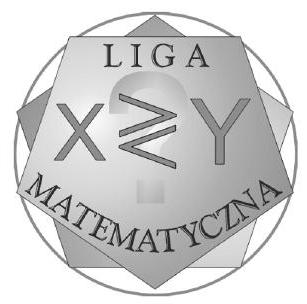
\includegraphics[max width=\textwidth]{2024_11_21_0e7bdb5465f22a653800g-1}
\end{center}

\section*{LIGA MATEMATYCZNA im. Zdzisława Matuskiego \\
 FINAŁ 26 marca 2019 \\
 SZKOŁA PODSTAWOWA \\
 (klasy IV - VI)}
\section*{ZADANIE 1.}
Sakiewka Adama zawiera monety srebrne i złote. Wszystkie monety srebrne są jednakowe i wszystkie monety złote są jednakowe. Dwie monety srebrne i cztery złote ważą łącznie 72 g , a dwie złote i cztery srebrne ważą 66 g . Oblicz łączną wagę trzech złotych i trzech srebrnych monet.

\section*{ZADANIE 2.}
Znajdź wszystkie liczby trzycyfrowe, których iloczyn cyfr jest liczbą pierwszą.

\section*{ZADANIE 3.}
Jedna z przekątnych dzieli pewien czworokąt na dwa trójkąty o obwodach 16 i 18, druga przekątna dzieli ten czworokąt na trójkąty o obwodach 12 i 20. Oblicz różnicę długości przekątnych tego czworokąta.

\section*{ZADANIE 4.}
Iloczyn trzech liczb naturalnych jest równy 36. Nawet gdy podamy ich sumę, nie będzie wiadomo, co to za liczby. Oblicz ich sumę.

\section*{ZADANIE 5.}
Numer szyfru do szkatułki Basi składa się z dziewięciu różnych cyfr i różnych od 0. Każde dwie kolejne cyfry szyfru różnią się o 3 lub 5. Pierwszą cyfrą kodu jest 3. Wyznacz przedostatnią cyfrę szyfru.


\end{document}